\chapter{Wykorzystane technologie}

Projekt został zrealizowany pod systemem Windows 10 oraz Mac OS X El Capitan. 

\section{C}
Z racji, iż sercem robota jest procesor z rodziny \textit{STM}, wybór technologii został ograniczony do języka C lub C++. Wybrano język C z powodów optymalizacyjnych oraz małego stopnia skomplikowania programu \cite{C}. 


Oprogramowanie zostało stworzone w środowisku \textit{Eclipse} z dodatkiem \textit{AC6} wspierającym platformę \textit{STM32}.

\subsection{Hardware Abstraction Layer}
\textit{HAL} jest biblioteką będącą wysokopoziomowym interfejsem służącym do konfiguracji peryferiów mikrokontrolera. Zdecydowano się na wyżej wspomnianą bilbiotekę z powodu bardzo przejrzystej dokumentacji oraz łatwości użytkowania. Dodatkowo użyto środowiska \textit{CubeMX}, które udostępnia graficzny interfejs pozwalający na stosunkowo łatwą oraz intuicyjną konfigurację procesora oraz wygenerowanie projektu w języku C wraz z~użyciem bibliotek HAL.

\newpage 

Rysunek ~\ref{fig:cubemx} przedstawia konfigurację peryferiów użytego procesora w środowisku CubeMX.   

\begin{figure}[H]
	\centering
		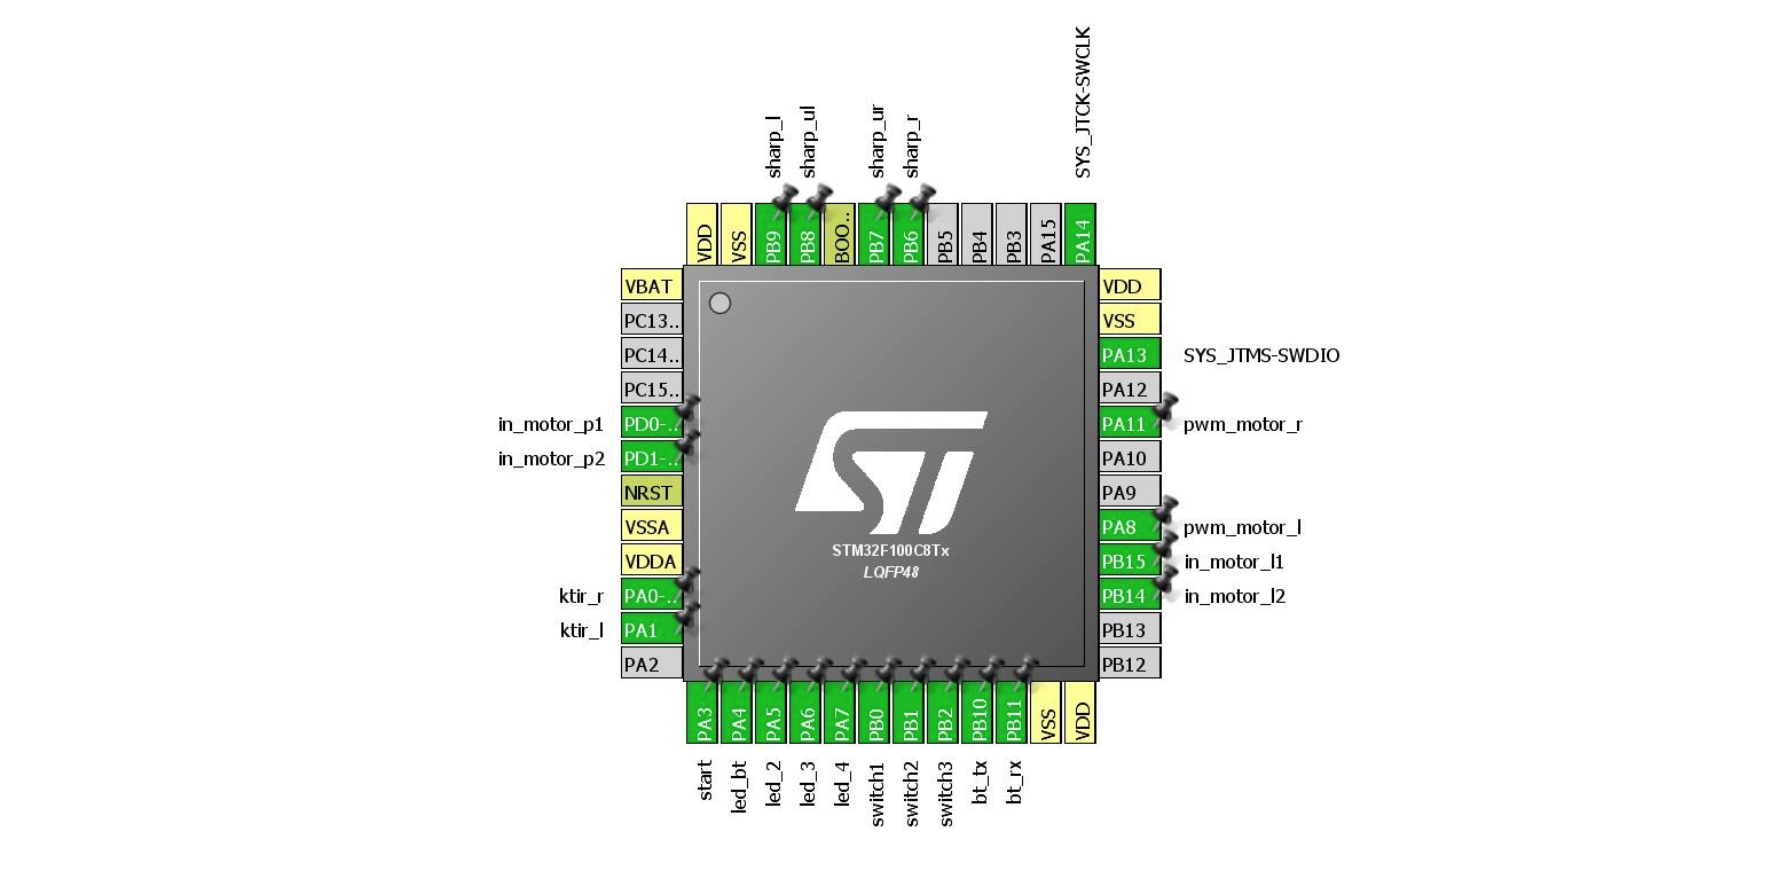
\includegraphics[width=\linewidth, scale=0.95]{pic02/cubemx}
	\caption{Konfiguracja peryferiów użytego procesora STM32F100C8T6B – LQFP48.}
	\label{fig:cubemx}	
\end{figure}

\newpage

\section{Swift}
\textit{Swift} jest językiem natywnym (następcą języka \textit{Objective–C}) zaprezentowanym przez \textit{Apple Inc.} w 2014 roku \cite{Swiftdoc}. Wykorzystywany jest do tworzenia oprogramowania na platformy \textit{macOS, iOS} oraz \textit{watchOS}. W pracy dyplomowej użyto wersji języka 3.0, ponieważ była to najnowsza wersja wspierana przez docelowe urządzenie, którym był telefon iPhone 5.

Środowiskiem użytym do tworzenia aplikacji mobilnej w technologii \textit{Swift} był \textit{Xcode}, którego dużym atutem jest występowanie graficznego interfejsu umożliwiającego tworzenie widoków aplikacji. Dzięki temu tworzenie aplikacji jest bardziej intuicyjne oraz pozwala na sprawne wprowadzanie zmian w tworzonych widokach \cite{Swift}.

Ilustracja ~\ref{fig:xcode} ukazuje środowisko Xcode wraz z widokami aplikacji oraz zależnościami między nimi.   

\begin{figure}[H]
	\centering
		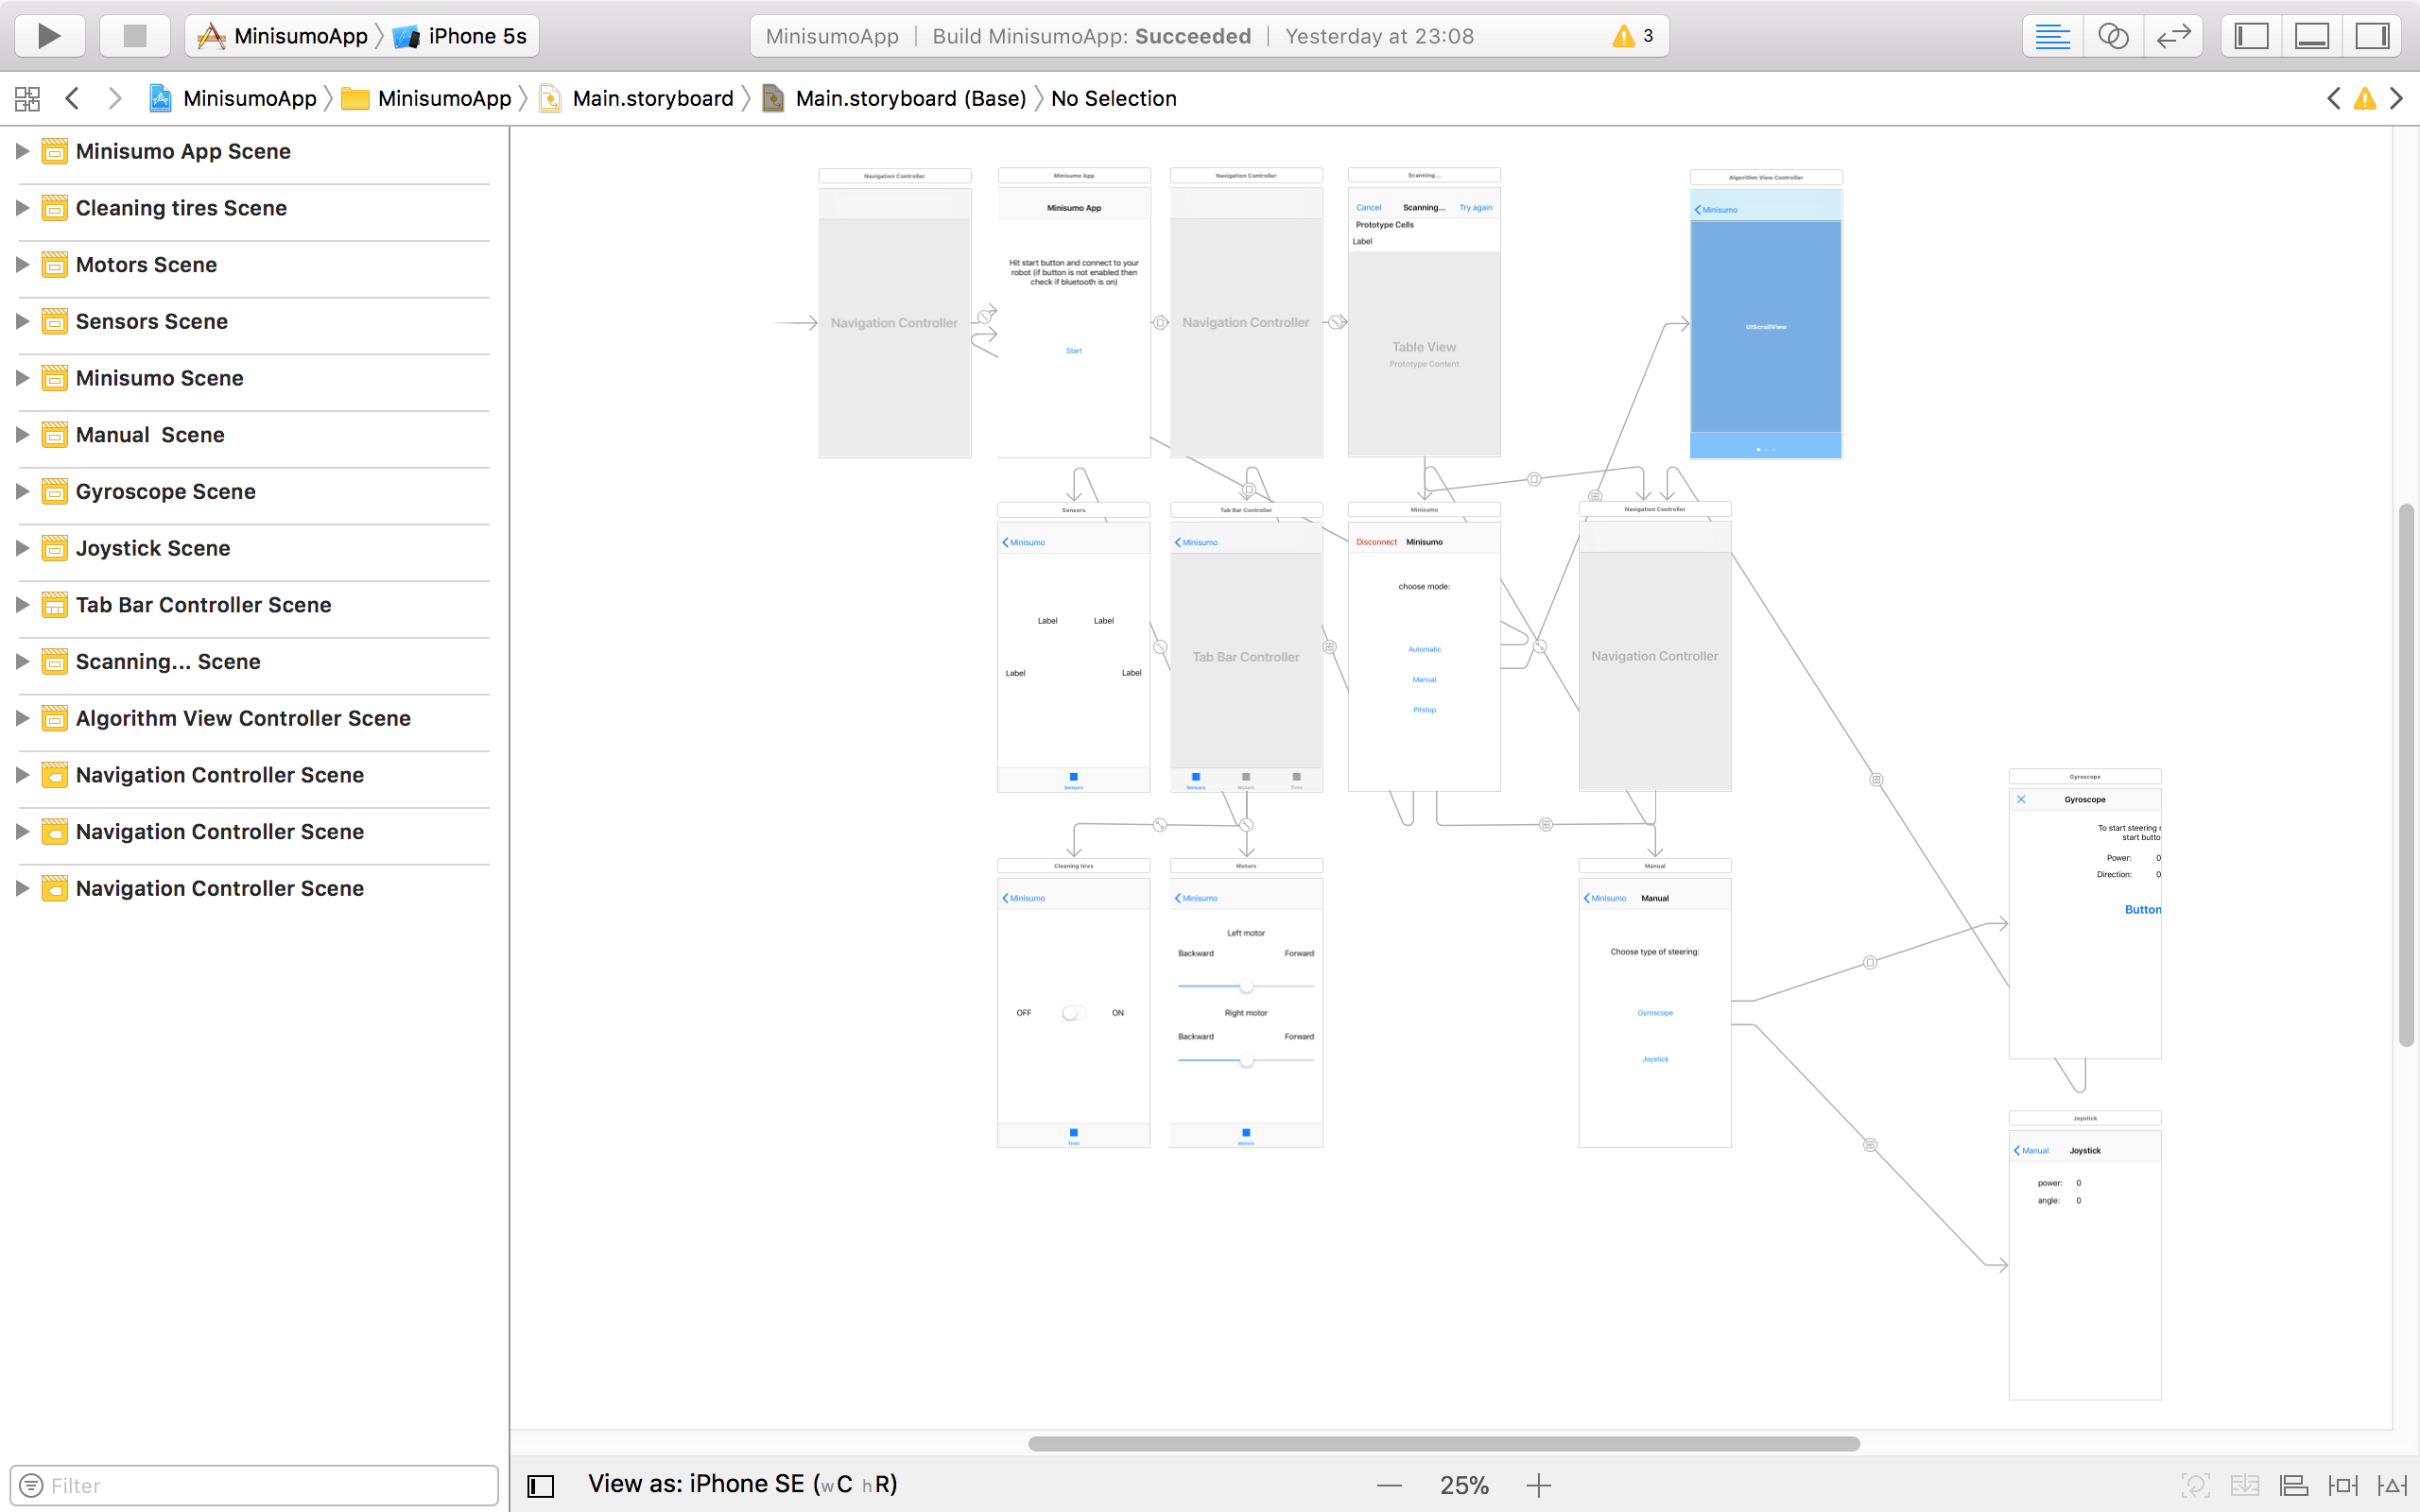
\includegraphics[width=0.75\linewidth]{pic02/xcode}
	\caption{Okno środowiska Xcode.}
	\label{fig:xcode}	
\end{figure}

\subsection{UIKit}
\textit{UIKit} jest platformą, która zapewnia infrastrukturę dla aplikacji. Udostępnia  architekturę widoku do implementacji interfejsu, obsługę zdarzeń, obsługę wielopunktowego dotyku, zarządza zasobami oraz interakcjami pomiędzy aplikacją a użytkownikiem. Dodatkowymi funkcjami są obsługa dokumentów, aplikacji oraz jej rozszerzeń, zarządzanie tekstem i wyświetlaniem \cite{AppleDocumentation}.

\index{UIView} \subsubsection{\lstinline$UIView$}
Widoki są podstawowymi elementami składowymi interfejsu użytkownika aplikacji, a klasa \textit{UIView} definiuje zachowania wspólne dla wszystkich widoków. Obiekt widoku renderuje zawartość w obrębie prostokąta obwiedni i obsługuje wszelkie interakcje z tą zawartością. 

\index{UITableView} \subsubsection{\lstinline$UITableView$}
\textit{UITableView} wyświetla listę pozycji w pojedynczej kolumnie. Jest podklasą \textit{UIScrollView}, która pozwala użytkownikowi przewijać tabelę, z tą różnicą, że przewijanie dozwolone jest wyłącznie w pionie. Komórki zawierające poszczególne elementy tabeli są obiektami \textit{UITableViewCell}. \textit{UITableView} używa wspomnianych obiektów do rysowania widocznych wierszy tabeli. Komórki mogą posiadać tytuły treści, obrazy oraz widoki akcesoriów, które mogą pełnić rolę elementów sterujących takich jak przełączniki i suwaki. 

\subsection{CoreBluetooth}
Platforma \textit{CoreBluetooth} dostarcza klasy niezbędne do komunikacji aplikacji z urządzeniami wyposażonymi w bezprzewodową komunikację Bluetooth.

\index{CBPeripheral} \subsubsection{\lstinline$CBPeripheral$}
Klasa \textit{CBPeripheral} reprezentuje zdalne urządzenia peryferyjne, których połączenie  aplikacja wykrywa za pośrednictwem instancji \textit{CBCentralManager}. Urządzenia peryferyjne są identyfikowane za pomocą unikalnych identyfikatorów (UUID) reprezentowanych przez obiekty NSUUID. 

\index{CBCentralManager} \subsubsection{\lstinline$CBCentralManager$}
Obiekty \textit{CBCentralManager} służą do zarządzania podłączonymi urządzeniami peryferyjnymi (reprezentowanymi przez obiekty \textit{CBPeripheral}). Pozwalają na skanowanie oraz wykrywanie zdalnych urządzeń.

\subsection{CoreGraphics}
Platforma \textit{CoreGraphics} oparta jest na zaawansowanym mechanizmie rysowania \textit{Quartz}. Zapewnia niskopoziomowe renderowanie 2D, zarządzanie wzorcami, gradientami oraz danymi obrazu. Dodatkowo pozwala na tworzenie oraz maskowanie obrazu, a także wyświetlanie i analizowanie dokumentów PDF. W pracy dyplomowej \textit{CoreGrapics} zostało wykorzystane do stworzenia wirtualnego dżojstiku służącego zdalnemu sterowaniu robotem minisumo. 

\subsection{CoreMotion}
Dostarcza dane dotyczące ruchu urządzenia na podstawie wbudowanego akcelerometru, żyroskopu, krokomierza, magnetometru, barometru itp. W aplikacji użyto wspomnianej platformy do sterowania ruchem robota za pomocą akcelerometru \cite{AppleDocumentation}.

\section{Arduino}
\textit{Arduino} jest platformą programistyczną przeznaczoną dla mikrokontrolerów z wbudowaną obsługą układów wejścia oraz wyjścia \cite{Arduino}. Język programowania \textit{Arduino} oparty jest na języku C/C++. Głównym atutem omawianej platformy jest szeroka społeczność, dokładna dokumentacja oraz łatwość prototypowania prostych układów. Jednakże omawiania platfomra nie jest zalecana w~przypadku złożonych projektów ze względu na wysokopoziomowość oraz niestabilność pracy.

Platforma została użyta do konfiguracji modułu Bluetooth za pomocą komend \textit{AT}. Skonfigurowano takie parametry jak nazwa urządzenia oraz liczbę symboli na sekundę (ang. \textit{baud rate}). Do tego celu użyto mikrokontrolera \textit{Arduino Mega 2560} oraz płytki stykowej wraz z przewodami połączeniowymi. Konfiguracja modułu była jednorazową czynnością, dlatego zdecydowano się na platformę \textit{Arduino} ze względu na wyżej wspomnianą szybkość oraz prostotę obsługi.
  

\begin{figure}[H]
	\centering
		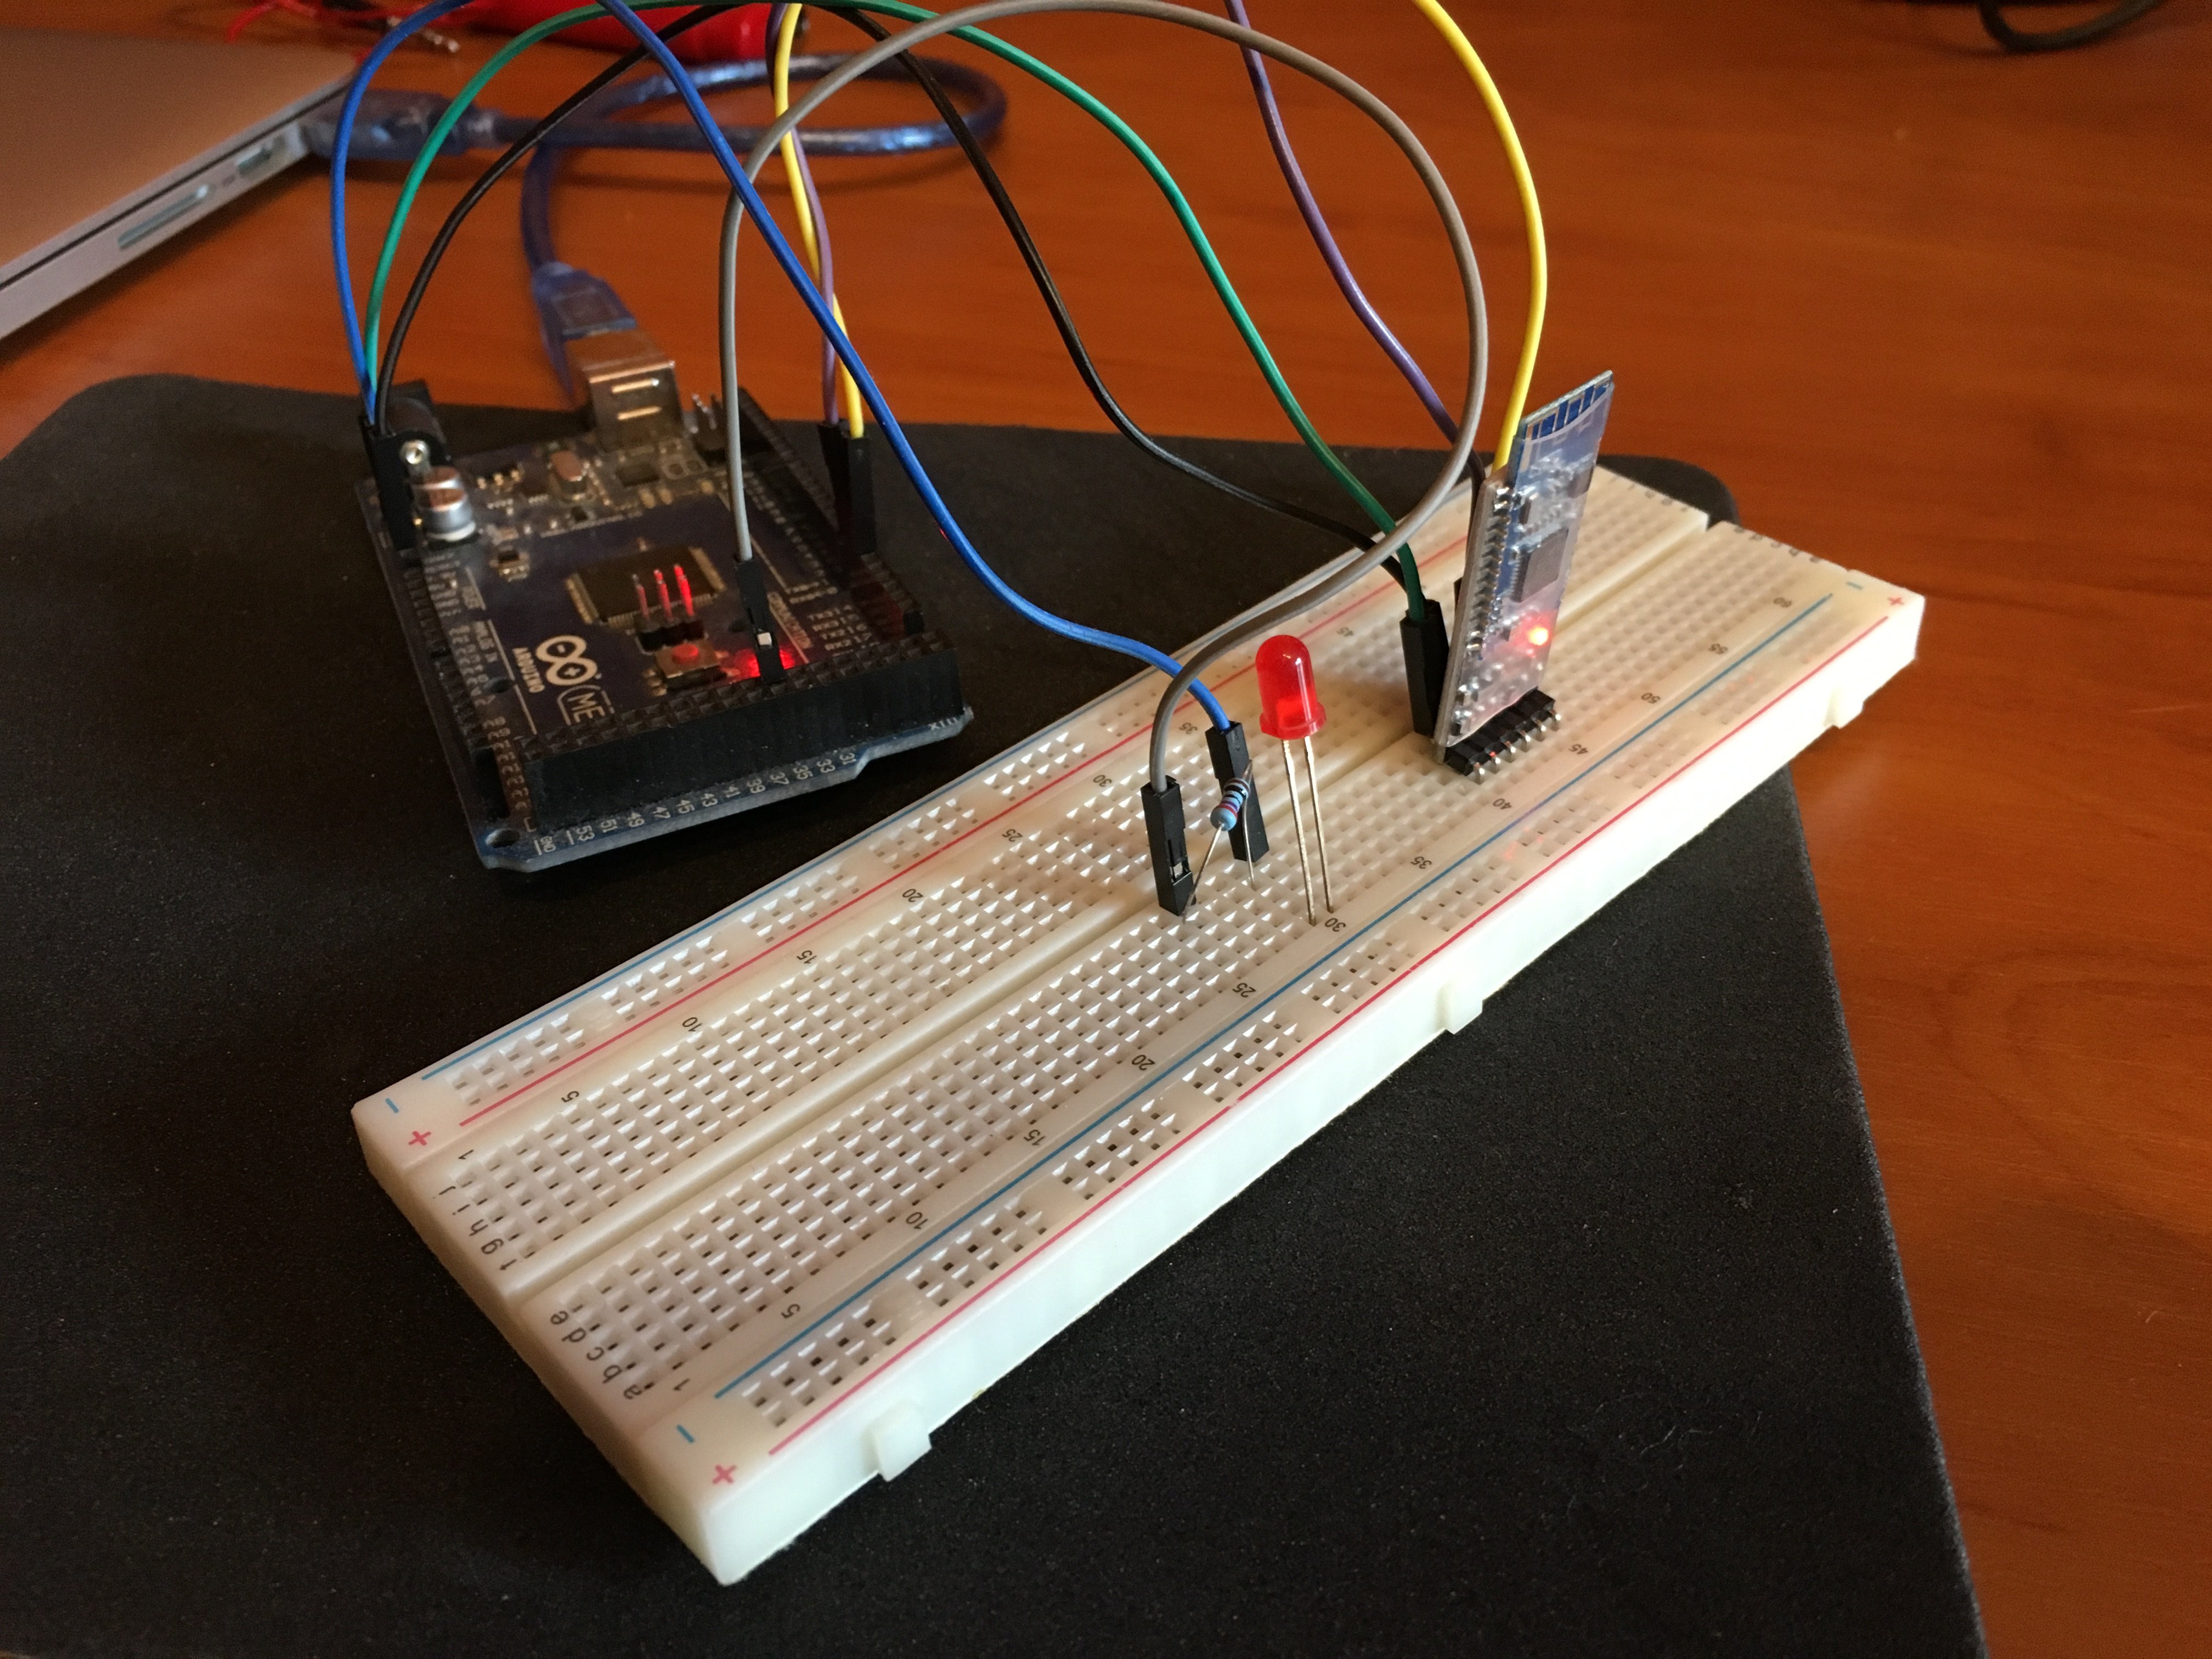
\includegraphics[width=0.75\linewidth]{pic02/arduino.JPG}
	\caption{Układ służący do konfiguracji modułu bluetooth.}
	\label{fig:arduino}	
\end{figure}

Rysunek ~\ref{fig:arduino} obrazuje układ \textit{Arduino Mega 2560} wraz z płytką stykową oraz podłączonym modułem bluetooth. Dodatkowo układ wyposażono w diodę mającą na celu sygnalizację poprawności wgrywania komend.

\newpage 

Listing \ref{arduinocode} przedstawia kod programu zapewniającego komunikację między komputerem a~modułem Bluetooth przy użyciu mikrokontrolera \textit{Arduino Mega 2560}. 

\begin{minipage}{\textwidth}
	\begin{lstlisting}[label=arduinocode,caption=Kod programu umożliwiającego konifugrację modułu Bluetooth HM–10.]
#include <SoftwareSerial.h>
 
int LEDPIN = 13;

void setup() {
  pinMode(LEDPIN, OUTPUT);
  Serial.begin(9600); // communication with computer
  Serial3.begin(9600); // communication with HM-10  
}
 
void loop() {
  if ( Serial3.available() ) {
    char dioda = Serial3.read();
    Serial.write(dioda);
    if (atoi(&dioda)==1) {
      digitalWrite(LEDPIN, HIGH);
    }
    
    if (atoi(&dioda)==0) {
      digitalWrite(LEDPIN, LOW);
    }
  }
  
  if ( Serial.available() ) {  Serial3.write( Serial.read() );  }  
}
	\end{lstlisting}
\end{minipage}
 
Za pomocą terminalu udostęnionego przez środowisko \textit{Arduino} możliwa jest komunikacja oraz konfiguracja modułu \textit{HM–10}. Dodatkowo program został rozszerzony o zapalanie oraz gaszenie diody LED w celu sprawdzenia poprawności połączenia. Jeżeli przy użyciu wyżej wspomnianego terminala zostanie wysłana wartość 1, powinna zapalić się dioda. W przypadku wysłania wartości 0, dioda powinna zgasnąć.


 
